% GNUPLOT: LaTeX picture with Postscript
\begingroup
  \makeatletter
  \providecommand\color[2][]{%
    \GenericError{(gnuplot) \space\space\space\@spaces}{%
      Package color not loaded in conjunction with
      terminal option `colourtext'%
    }{See the gnuplot documentation for explanation.%
    }{Either use 'blacktext' in gnuplot or load the package
      color.sty in LaTeX.}%
    \renewcommand\color[2][]{}%
  }%
  \providecommand\includegraphics[2][]{%
    \GenericError{(gnuplot) \space\space\space\@spaces}{%
      Package graphicx or graphics not loaded%
    }{See the gnuplot documentation for explanation.%
    }{The gnuplot epslatex terminal needs graphicx.sty or graphics.sty.}%
    \renewcommand\includegraphics[2][]{}%
  }%
  \providecommand\rotatebox[2]{#2}%
  \@ifundefined{ifGPcolor}{%
    \newif\ifGPcolor
    \GPcolorfalse
  }{}%
  \@ifundefined{ifGPblacktext}{%
    \newif\ifGPblacktext
    \GPblacktexttrue
  }{}%
  % define a \g@addto@macro without @ in the name:
  \let\gplgaddtomacro\g@addto@macro
  % define empty templates for all commands taking text:
  \gdef\gplbacktext{}%
  \gdef\gplfronttext{}%
  \makeatother
  \ifGPblacktext
    % no textcolor at all
    \def\colorrgb#1{}%
    \def\colorgray#1{}%
  \else
    % gray or color?
    \ifGPcolor
      \def\colorrgb#1{\color[rgb]{#1}}%
      \def\colorgray#1{\color[gray]{#1}}%
      \expandafter\def\csname LTw\endcsname{\color{white}}%
      \expandafter\def\csname LTb\endcsname{\color{black}}%
      \expandafter\def\csname LTa\endcsname{\color{black}}%
      \expandafter\def\csname LT0\endcsname{\color[rgb]{1,0,0}}%
      \expandafter\def\csname LT1\endcsname{\color[rgb]{0,1,0}}%
      \expandafter\def\csname LT2\endcsname{\color[rgb]{0,0,1}}%
      \expandafter\def\csname LT3\endcsname{\color[rgb]{1,0,1}}%
      \expandafter\def\csname LT4\endcsname{\color[rgb]{0,1,1}}%
      \expandafter\def\csname LT5\endcsname{\color[rgb]{1,1,0}}%
      \expandafter\def\csname LT6\endcsname{\color[rgb]{0,0,0}}%
      \expandafter\def\csname LT7\endcsname{\color[rgb]{1,0.3,0}}%
      \expandafter\def\csname LT8\endcsname{\color[rgb]{0.5,0.5,0.5}}%
    \else
      % gray
      \def\colorrgb#1{\color{black}}%
      \def\colorgray#1{\color[gray]{#1}}%
      \expandafter\def\csname LTw\endcsname{\color{white}}%
      \expandafter\def\csname LTb\endcsname{\color{black}}%
      \expandafter\def\csname LTa\endcsname{\color{black}}%
      \expandafter\def\csname LT0\endcsname{\color{black}}%
      \expandafter\def\csname LT1\endcsname{\color{black}}%
      \expandafter\def\csname LT2\endcsname{\color{black}}%
      \expandafter\def\csname LT3\endcsname{\color{black}}%
      \expandafter\def\csname LT4\endcsname{\color{black}}%
      \expandafter\def\csname LT5\endcsname{\color{black}}%
      \expandafter\def\csname LT6\endcsname{\color{black}}%
      \expandafter\def\csname LT7\endcsname{\color{black}}%
      \expandafter\def\csname LT8\endcsname{\color{black}}%
    \fi
  \fi
    \setlength{\unitlength}{0.0500bp}%
    \ifx\gptboxheight\undefined%
      \newlength{\gptboxheight}%
      \newlength{\gptboxwidth}%
      \newsavebox{\gptboxtext}%
    \fi%
    \setlength{\fboxrule}{0.5pt}%
    \setlength{\fboxsep}{1pt}%
\begin{picture}(8162.00,5442.00)%
    \gplgaddtomacro\gplbacktext{%
      \csname LTb\endcsname%%
      \put(946,704){\makebox(0,0)[r]{\strut{}0.0}}%
      \put(946,1080){\makebox(0,0)[r]{\strut{}1.0}}%
      \put(946,1457){\makebox(0,0)[r]{\strut{}2.0}}%
      \put(946,1833){\makebox(0,0)[r]{\strut{}3.0}}%
      \put(946,2210){\makebox(0,0)[r]{\strut{}4.0}}%
      \put(946,2586){\makebox(0,0)[r]{\strut{}5.0}}%
      \put(946,2963){\makebox(0,0)[r]{\strut{}6.0}}%
      \put(946,3339){\makebox(0,0)[r]{\strut{}7.0}}%
      \put(946,3715){\makebox(0,0)[r]{\strut{}8.0}}%
      \put(946,4092){\makebox(0,0)[r]{\strut{}9.0}}%
      \put(946,4468){\makebox(0,0)[r]{\strut{}10.0}}%
      \put(946,4845){\makebox(0,0)[r]{\strut{}11.0}}%
      \put(946,5221){\makebox(0,0)[r]{\strut{}12.0}}%
      \put(1078,484){\makebox(0,0){\strut{}0.00}}%
      \put(1747,484){\makebox(0,0){\strut{}0.10}}%
      \put(2415,484){\makebox(0,0){\strut{}0.20}}%
      \put(3084,484){\makebox(0,0){\strut{}0.30}}%
      \put(3753,484){\makebox(0,0){\strut{}0.40}}%
      \put(4422,484){\makebox(0,0){\strut{}0.50}}%
      \put(5090,484){\makebox(0,0){\strut{}0.60}}%
      \put(5759,484){\makebox(0,0){\strut{}0.70}}%
      \put(6428,484){\makebox(0,0){\strut{}0.80}}%
      \put(7096,484){\makebox(0,0){\strut{}0.90}}%
      \put(7765,484){\makebox(0,0){\strut{}1.00}}%
      \put(3352,3715){\makebox(0,0)[l]{\strut{}\small Capacity factor = 0.328}}%
    }%
    \gplgaddtomacro\gplfronttext{%
      \csname LTb\endcsname%%
      \put(198,2962){\rotatebox{-270}{\makebox(0,0){\strut{}Normalised mean absolute error, \%}}}%
      \put(4421,154){\makebox(0,0){\strut{}Battery energy capacity, p.u.}}%
      \csname LTb\endcsname%%
      \put(5389,4938){\makebox(0,0)[l]{\strut{}\small 30-minute control horizon}}%
      \csname LTb\endcsname%%
      \put(5389,4718){\makebox(0,0)[l]{\strut{}\small 60-minute control horizon}}%
      \csname LTb\endcsname%%
      \put(5389,4498){\makebox(0,0)[l]{\strut{}\small 90-minute control horizon}}%
    }%
    \gplbacktext
    \put(0,0){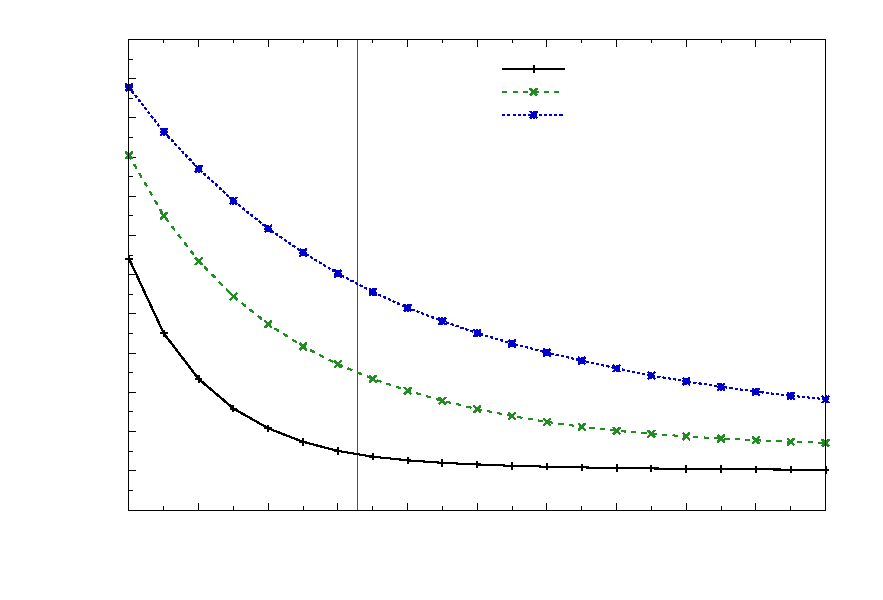
\includegraphics{plot_wind_bess_nmae_hrzn}}%
    \gplfronttext
  \end{picture}%
\endgroup
